\documentclass[varwidth, border=5pt]{standalone}

% Inspiration:
% ISBN: 978-0-241-38519-7, pp. 92--94
%
% See also:
% github.com/jakewilliami/tex-macros/blob/de32ec67/examples/confusion-matrix.tex
%
% A note on the distinction between tactics and strategy:
% reddit.com/r/explainlikeimfive/comments/1ceceob/comment/l1hl09c

\usepackage[utf8]{inputenc}
\usepackage[T1]{fontenc}
\usepackage{tikz}
\usepackage{amsmath}
\usetikzlibrary{calc, positioning}
\usepackage{xcolor}

% Em dash
\usepackage{etoolbox}
\def\emdash{\discretionary{}{}{\kern 0.1em}---\discretionary{}{}{\kern 0.1em}}

% Colours (mimicking Excel highlighted cells)
\definecolor{bgred}{RGB}{255, 199, 206}
\definecolor{fgred}{RGB}{156, 0, 6}
\definecolor{bggreen}{RGB}{198, 239, 206}
\definecolor{fggreen}{RGB}{0, 97, 0}
\definecolor{bgyellow}{RGB}{255, 235, 156}
\definecolor{fgyellow}{RGB}{156, 101, 0}

% Element styles
\newlength{\cellsz}\setlength{\cellsz}{10em}
\tikzstyle{cell}=[draw, text width=\cellsz, minimum height=\cellsz, align=center]
\tikzstyle{good}=[cell, fill=bggreen, text=fggreen]
\tikzstyle{bad}=[cell, fill=bgred, text=fgred]
\tikzstyle{ok}=[cell, fill=bgyellow, text=fgyellow]
\tikzstyle{standard}=[font=\normalsize]
\tikzstyle{label}=[standard]
\tikzstyle{total}=[standard]
\tikzstyle{note}=[font=\footnotesize, text width=20em, align=justify, xshift=3em]

\begin{document}

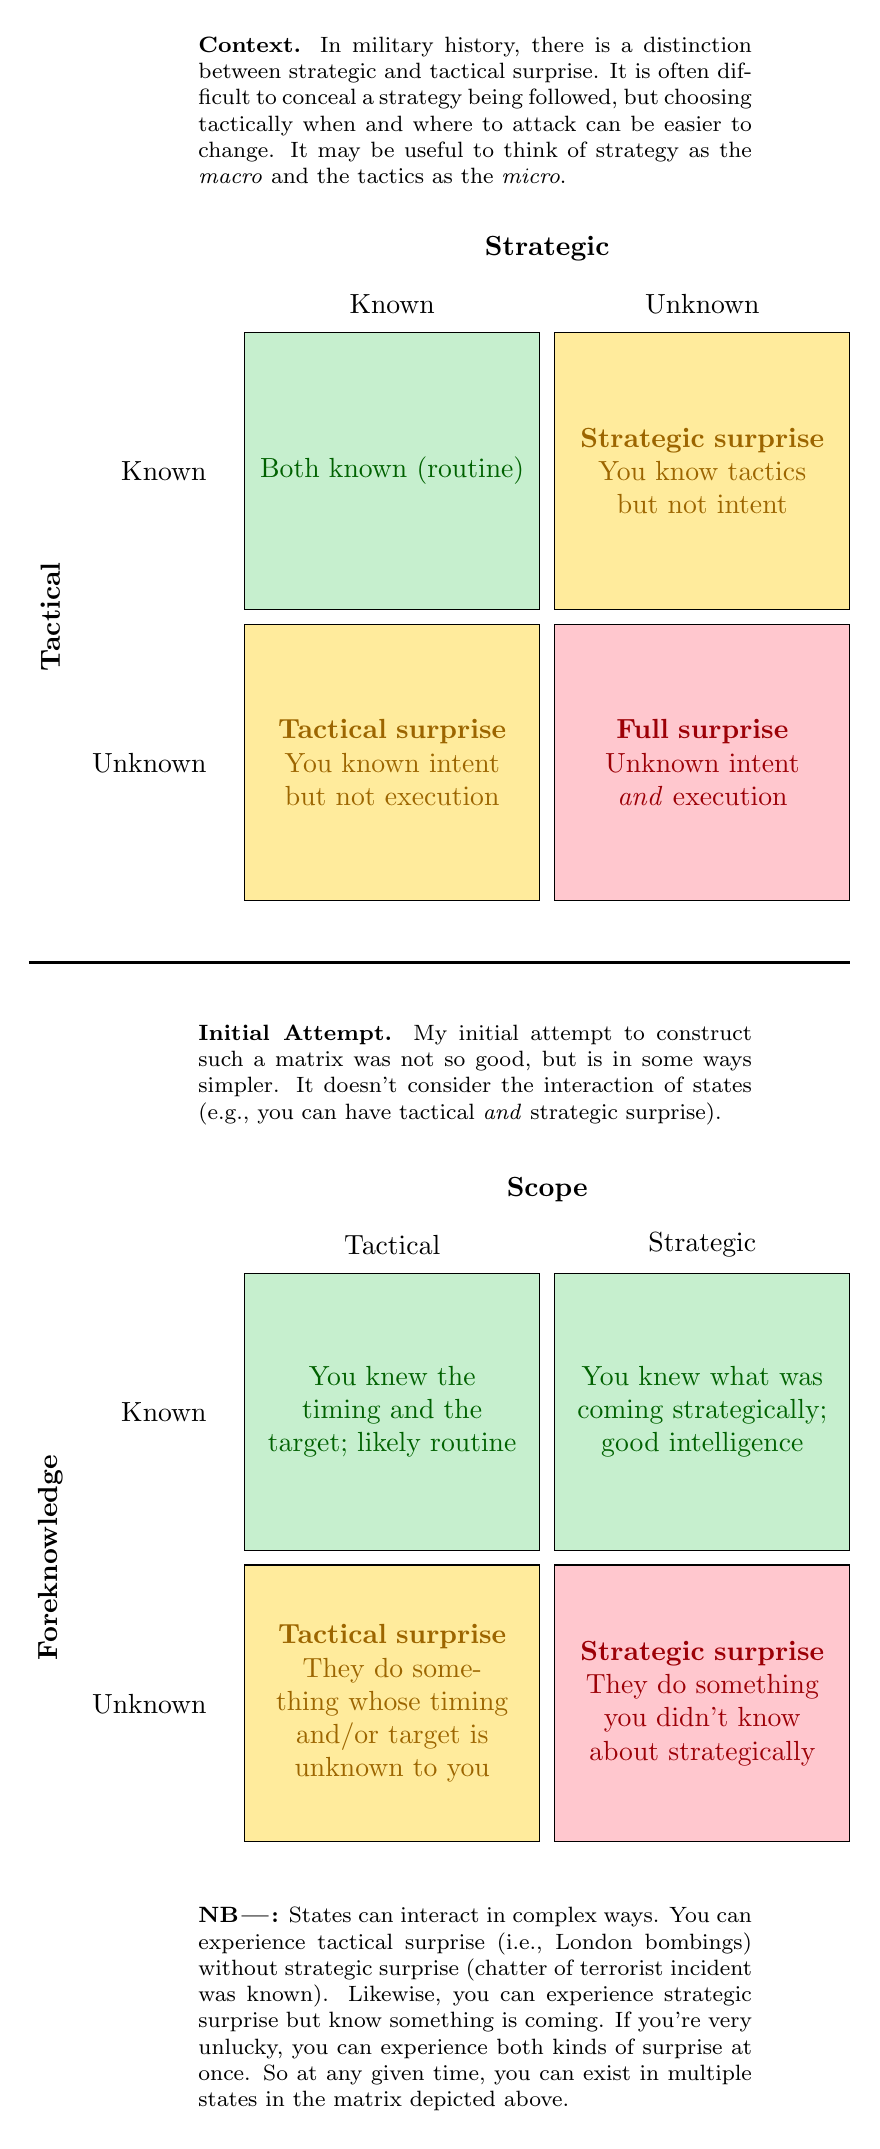
\begin{tikzpicture}

%%%%%%%%%%%%%%%%%
% Corrected matrix                     %
%%%%%%%%%%%%%%%%%

\begin{scope}

% Define matrix blocks
\node[good] (bothknown) at (0,0) {Both known (routine)};
\node[ok, right=0.5em of bothknown] (strategicsurprise) {\textbf{Strategic surprise}\\You know tactics but not intent};
\node[ok, below=0.5em of bothknown] (tacticalsurprise) {\textbf{Tactical surprise}\\You known intent but not execution};
\node[bad, right=0.5em of tacticalsurprise] (fullsurprise) {\textbf{Full surprise}\\Unknown intent \emph{and} execution};

% Axis labels
\node[label, rotate=00] at ([yshift=3em]$(bothknown.north)!0.5!(strategicsurprise.north)$) {\textbf{Strategic}};
\node[label, rotate=90] at ([xshift=-7em]$(bothknown.west)!0.5!(tacticalsurprise.west)$)  {\textbf{Tactical}};

% Individual cell axis labels
\node[label, anchor=center] at ([yshift=1em]bothknown.north) {Known};
\node[label, anchor=center] at ([yshift=1em]strategicsurprise.north) {Unknown};
\node[label, anchor=east] at ([xshift=-1em]bothknown.west) {Known};
\node[label, anchor=east] at ([xshift=-1em]tacticalsurprise.west) {Unknown};

% Notes
\node[note, above=5em of bothknown.north] (foreword)
    {\textbf{Context.}  In military history, there is a distinction between strategic and tactical surprise.  It is often difficult to conceal a strategy being followed, but choosing tactically when and where to attack can be easier to change.  It may be useful to think of strategy as the \emph{macro} and the tactics as the \emph{micro}.};  % NOTE: Similar to IOCs vs TTPs?  Harder to change chain of process, but easy to change domains

\end{scope}

%%%%%%%%%%%%%%%%%
% First attempt                           %
%%%%%%%%%%%%%%%%%

\begin{scope}[yshift=-34em]

% Define matrix blocks
\node[good] (TP) at (0,0) {You knew the timing and the target; likely routine};
\node[good, right=0.5em of TP] (FN) {You knew what was coming strategically; good intelligence}; % planned % TODO: is this 
\node[ok, below=0.5em of TP] (FP) {\textbf{Tactical surprise}\\They do something whose timing and/or target is unknown to you};
\node[bad, right=0.5em of FP] (TN) {\textbf{Strategic surprise}\\They do something you didn't know about strategically};

% Axis labels
\node[label, rotate=00] at ([yshift=3em]$(TP.north)!0.5!(FN.north)$) {\textbf{Scope}};  % TODO: is this a good name for this axis?
\node[label, rotate=90] at ([xshift=-7em]$(TP.west)!0.5!(FP.west)$)  {\textbf{Foreknowledge}};  % TODO: is this a good name for this axis?  "Known?"  I had "Detection" for "Detected" and "Silent", so I could rename to "Expectation"

% Individual cell axis labels
\node[label, anchor=center] at ([yshift=1em]TP.north) {Tactical};
\node[label, anchor=center] at ([yshift=1em]FN.north) {Strategic};
\node[label, anchor=east] at ([xshift=-1em]TP.west) {Known};  % Should I rename these to known vs unknown?
\node[label, anchor=east] at ([xshift=-1em]FP.west) {Unknown};

% Notes
\node[note, above=5em of TP.north] (foreword)
    {\textbf{Initial Attempt.}  My initial attempt to construct such a matrix was not so good, but is in some ways simpler.  It doesn't consider the interaction of states (e.g., you can have tactical \emph{and} strategic surprise).};

\node[note, below=2em of FP.south] (NB)
    {\textbf{NB\emdash:} States can interact in complex ways.  You can experience tactical surprise (i.e., London bombings) without strategic surprise (chatter of terrorist incident was known).  Likewise, you can experience strategic surprise but know something is coming.  If you're very unlucky, you can experience both kinds of surprise at once.  So at any given time, you can exist in multiple states in the matrix depicted above.};

\end{scope}

%%%%%%%%%%%%%%%%%
% Separator                               %
%%%%%%%%%%%%%%%%%

\coordinate (midY) at ($(tacticalsurprise.south)!0.5!(TP.north)$);
\draw[thick]
  ([yshift=4.5em]midY -| current bounding box.west) --
  ([yshift=4.5em]midY -| current bounding box.east);

\end{tikzpicture}

\end{document}
